\documentclass[border=10pt]{standalone}
\usepackage{amsmath,amssymb,tikz}
\usepackage[svgnames]{xcolor}

\pagecolor{LightYellow}
\color{DarkSlateGray}

\begin{document}
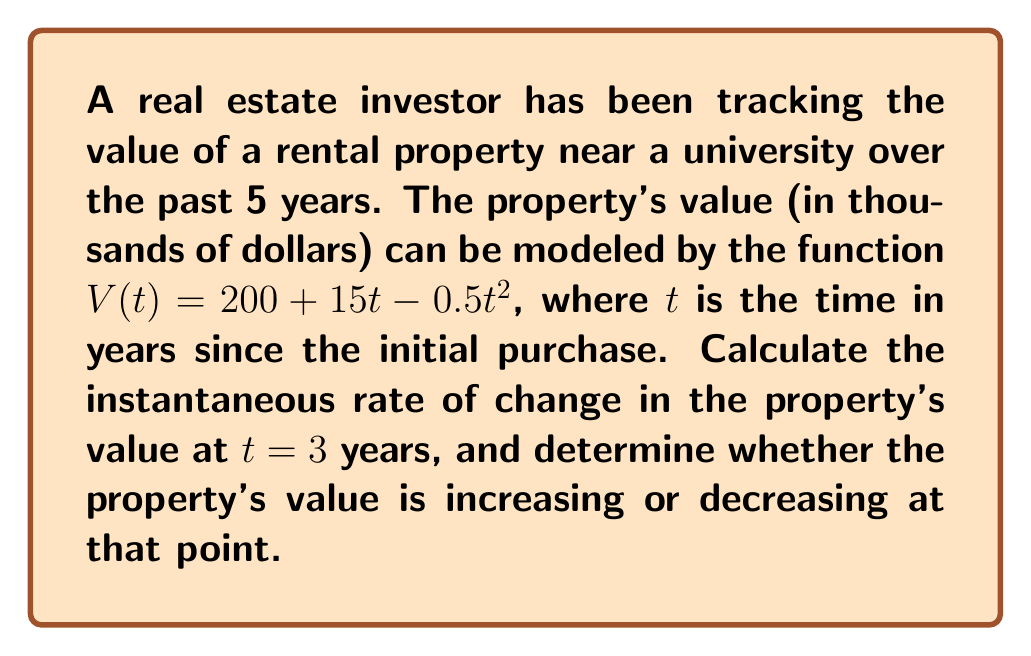
\begin{tikzpicture}
\node[draw=Sienna,line width=2pt,rounded corners,fill=Bisque,inner sep=20pt] {
\begin{minipage}{0.9\textwidth}
\Large\sffamily\bfseries
A real estate investor has been tracking the value of a rental property near a university over the past 5 years. The property's value (in thousands of dollars) can be modeled by the function $V(t) = 200 + 15t - 0.5t^2$, where $t$ is the time in years since the initial purchase. Calculate the instantaneous rate of change in the property's value at $t = 3$ years, and determine whether the property's value is increasing or decreasing at that point.
\end{minipage}
};
\end{tikzpicture}
\end{document}